\documentclass[12pt]{report}

% packages used for many things
\usepackage[utf8]{inputenc}
\usepackage[english]{babel}
\usepackage{hyperref}
\hypersetup{colorlinks=true, linkcolor=blue, filecolor=magenta, urlcolor=cyan}
\urlstyle{same}
% package used for the enumeration
\usepackage{enumitem}
% packages used to write more symbols and text in math mode
\usepackage{amsmath}
\usepackage{mathtools}
\usepackage{amsfonts} 
\usepackage{amssymb}
\usepackage{MnSymbol}
\usepackage{csquotes}
\usepackage{arydshln}
\usepackage{algorithm}
\usepackage{algorithmic}
\usepackage{extarrows}
\usepackage{tikz}


% \usepackage{geometry}
%  \geometry{
%  a4paper,
%  total={170mm,257mm},
%  left=20mm,
%  top=15mm,
%  }


% for images
\usepackage{graphicx}
\graphicspath{{./images/}}

% qed black square
\newcommand*{\QEDA}{\hfill\ensuremath{\blacksquare}}
% xor symbol
\newcommand*\xor{\oplus}

\title{Artificial Intelligence II \\ Assignment 3 Report}
\author{Andreas - Theologos Spanopoulos (sdi1700146@di.uoa.gr)}
\date{December 27, 2020}


% ----------------    START OF DOCUMENT    ------------ %
\begin{document}
\maketitle

% ------------------------------      REGURAL MODEL       ----------------------------------- %
\section*{Regular Model}
The Notebook (AI2\_HW3.ipynb) is properly commented, so I will not go into deep
details regarding most matters.
\bigskip

% ------------------------------      PREPROCESSING       ----------------------------------- %
\subsection*{Preprocessing}
Every sentence from the dataset in preprocessed using the "main\_pipeline" function defined in
the preprocessing.py file. It removes urls, twitter tags, most useless punctuation, numbers,
multiple whitespace and it converts every letter to lowercase. Some sentences turned out to have
a length of 0 after being preprocessed, so they got removed fromt the dataset.
\bigskip

% ------------------------------      ARCHITECTURE       ----------------------------------- %
\subsection*{Architecture}
The architecture of the final model is pretty straightforward:

\begin{align*}
    \text{Input X} &\;\xRightarrow[]{\text{Embedding}}\; \text{X embedded} \\[1.5ex]
                   &\;\xRightarrow[]{\text{RNN Cell}}\; \text{RNN output,
                                                    \underline{last hidden state output}} \\[1.5ex]
                   &\;\xRightarrow[]{\text{Dropout}}\; \text{Dropout output} \\[1.5ex]
                   &\;\xRightarrow[]{\text{FC Layer}}\; \text{FC output} \\[1.5ex]
                   &\;\xRightarrow[]{\text{Sigmoid}}\; \text{logit (model output)}
\end{align*}
Note that from the RNN only the last hidden state is used.
\clearpage

% ------------------------------      HYPERPARAMETERS       ----------------------------------- %
\subsection*{Hyperparameters}
The hyperparameters found to be optimal (using a Grid Seach and many trial/errors) for the model
are:
\bigskip

\begin{itemize}
    \item Batch Size = 32
    \item Max Vocabulary Size = 25000
    \item Epochs = 5
    \item Learnign Rate = 0.0075
    \item Clipping amount = 10
    \item GloVe = glove.twitter.27B.100d
    \item RNN Type = LSTM
    \item Number of Stacked RNNs = 1
    \item Skip Connections = False
    \item Embedding Dimension = 100 (from GloVe)
    \item Vocabulary Size = length(vocabulary)
    \item Hidden Dimension = 512
    \item RNN Layers = 2
    \item RNN Dropout = 0.1
    \item Dropout Rate = 0,1
    \item Bidirectional = True
    \item Optimizer = Adam
    \item Loss = Binary Cross Entropy
\end{itemize}
\clearpage

% ------------------------------      PERFORMANCE       ----------------------------------- %
\subsection*{Performance}
The performance of the model using the above hyperparameters yields:
\begin{itemize}
    \item Training Loss: 0.54, Validation Loss: 0.52
    \item Training Accuracy: 0.72, Validation Accuracy: 0.74
    \item Training F1 Score: 0.71, Validation F1 Score: 0.74
\end{itemize}
\bigskip

\noindent The ROC Curve for the model on the Test set, is:
\bigskip
\bigskip

\hspace*{-2.0cm}
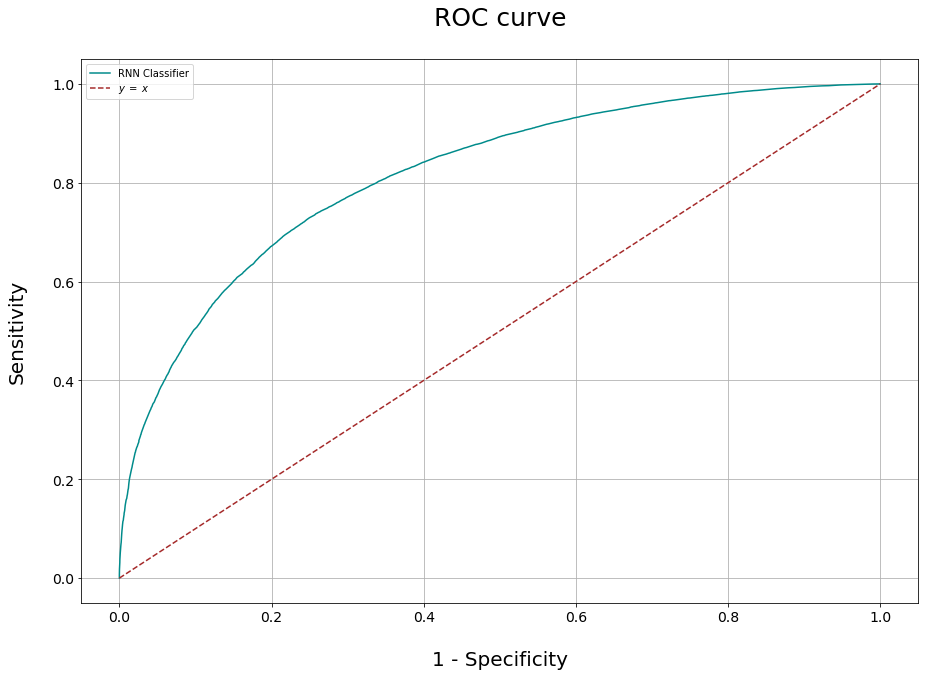
\includegraphics[scale=0.45]{roc1.png}
\smallskip


\clearpage
% ------------------------------      EXPERIMENTS       ----------------------------------- %
\subsection*{Experiments}
The following hyperparameters/experiments/modifications were tried to the model and its
architecture:
\smallskip

\begin{itemize}
    \item Stacking more RNN (LSTM and GRU) layers (2 were tried) did not lead to any
        significant improvement. In the contrary, it slowed down the training process.
    \item Skip Connections only make sense for 2+ RNN stacked layers. It was tried, bu since
        the shape of each batch size is incosistent, padding was required, something that I
        tried to avoid.
    \item Number of Hidden Layers: 1, 2, 3 and 4 were tried. 1 Hidden layer performed the
        worst, but was faster during training. 2 and 3 seems to be performing the best, with
        models using 3 hidden layers showing a slight improvement.
    \item LSTM and GRU recurrent networks were tried. GRU was faster during training, but
        scored always 1-2\% less F1 score in each epoch, compared to LSTM.
    \item Gradient Clipping was tried with values in the set \{5, 10, 50, 100\}. No
        difference was noticed. Also, no clipping was applied, which led to increase in
        the losses.
    \item Dropout was tried with values from 0.0 up to 0.5. Around 0.2 was found to give
        the best model, and it didn't make sense to increase the dropout rate as the model
        was not overfitting.
    \item Learning rates in the range [0.1, 0.0001] were tried. 0.001 works better in the
        begginign but it plateaus from the first epoch. 0.0001 starts lower but climbs to
        a better value after some epochs.
    \item Fine tuning the Embedding layer was tried, that is, to freeze the embedding layer
        in the first few epochs and then unfreeze it. No improvements were shown.
    \item Chaning the Max Vocabulary size in the range [15000, 30000] did not have any effects.
    \item Adding weight decay did not improve anything, as the model was not overfitting.
    \item Using bidirectional RNNs improves Accuracy and F1 Score by 5\%.
    \item Different Train sizes were tried, from 80\% to 95\% of the whole dataset. 90\% is
        believed to preserve an acceptable balance, so it was chosen as the default split.
    \item Different methods of preprocessing were tried and removed. Very simple preprocessing
        pipelines (remove urls, keep only alphanumerical values and convert to lowecase) decrease
        the model performance, but also very thorough ones (everything mentioned in page 1) remove
        valuable information from the dataset. I believe this is the main reason for why the
        model was not able to perform better. I will try more configurations of preprocessing
        methods before submitting.
\end{itemize}
\bigskip

% ------------------------------      COMPARISON       ----------------------------------- %
\subsection*{Comparison with the best model from the previous assignment}
The best model from assignment 2 (NN with tfidf) reached a peak score of 0.78 Accuracy and F1.
Compared to this model, is perfomed better, but it showed signs of overfitting. This model on
the other hand, reaches 0.74 on the same metrics, but it doesn't overfit. Its training time
is a bit slower though. Also, the ROC curve of this model is has smaller area than that of
the second assignment. So yeap, the previous model performs better in general, but it
doesn't have a window of improvement. On the contrary, we will see that once adding
Attention to the current model, its performance improves significantly.


\clearpage
% ------------------------------      ATTENTION MODEL       ----------------------------------- %
\section*{Attention Model}
The Notebook (AI2\_HW3\_Bonus.ipynb) is properly commented, so I will not go into deep
details regarding most matters. The paper which describes the implementation, is
the: \href{https://arxiv.org/abs/1703.03130}{A Structured Self-attentive Sentence Embedding}.
\bigskip

% ------------------------------      PREPROCESSING       ----------------------------------- %
\subsection*{Preprocessing}
Same as in the first model.
\bigskip

% ------------------------------      ARCHITECTURE       ----------------------------------- %
\subsection*{Architecture}
The architecture of the attention model is pretty straightforward:

\begin{align*}
    \text{Input X} &\;\xRightarrow[]{\text{Embedding}}\; \text{X embedded} \\[1.35ex]
                   &\;\xRightarrow[]{\text{RNN Cell}}\; \text{\underline{RNN output},
                                                    last hidden state output} \\[1.35ex]
                   &\;\xRightarrow[]{\text{Attention}}\; \text{Attention Network output} \\[1.35ex]
                   &\;\xRightarrow[]{\text{Dropout}}\; \text{Dropout output} \\[1.35ex]
                   &\;\xRightarrow[]{\text{FC Layer}}\; \text{FC output} \\[1.35ex]
                   &\;\xRightarrow[]{\text{Sigmoid}}\; \text{logit (model output)}
\end{align*}
Note that to the Attention Network we feed the whole RNN output (all the hidden states).
\clearpage


% ------------------------------      HYPERPARAMETERS       ----------------------------------- %
\subsection*{Hyperparameters}
Using the same hyperparameters as the previous model does not yield good results, as the new
model overfits early, plus it takes a lot of time for training. The hyperparameters below
seem to be yielding the best results for the attention model:
\bigskip

\begin{itemize}
    \item Batch Size = 128
    \item Max Vocabulary Size = 25000
    \item Epochs = 15
    \item Learnign Rate = 0.003
    \item Clipping amount = 10
    \item GloVe = glove.twitter.27B.100d
    \item RNN Type = LSTM
    \item Number of Stacked RNNs = 1
    \item Skip Connections = False
    \item Embedding Dimension = 100 (from GloVe)
    \item Vocabulary Size = length(vocabulary)
    \item Hidden Dimension = 256
    \item RNN Layers = 2
    \item RNN Dropout = 0.2
    \item Dropout Rate = 0,2
    \item Bidirectional = True
    \item Optimizer = Adam
    \item Loss = Binary Cross Entropy
    \item Max Sentence Length = 40
    \item Context Dimension ($d_a$) = 2 * Hidden Dimension = 512
\end{itemize} \clearpage


% ------------------------------      PERFORMANCE       ----------------------------------- %
\subsection*{Performance}
The performance of the attention model using the above hyperparameters yields:
\begin{itemize}
    \item Training Loss: 0.44, Validation Loss: 0.43
    \item Training Accuracy: 0.79, Validation Accuracy: 0.80
    \item Training F1 Score: 0.79, Validation F1 Score: 0.80
\end{itemize}
\bigskip

\noindent The ROC Curve for the model on the Test set, is:
\bigskip
\bigskip

\hspace*{-2.0cm}
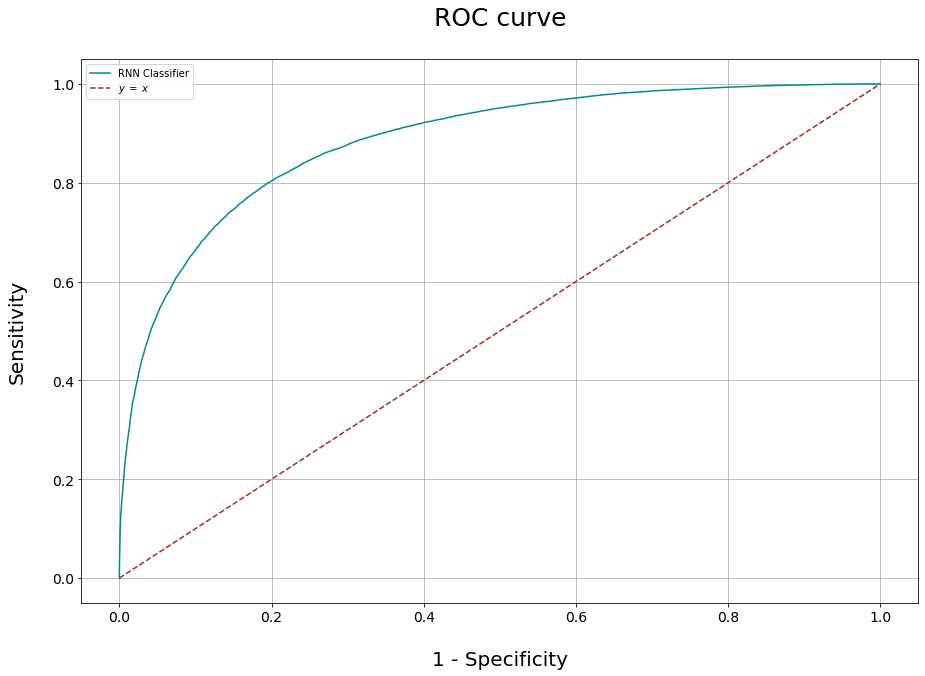
\includegraphics[scale=0.45]{roc2.png}
\clearpage


% ------------------------------      CONCLUSIONS       ----------------------------------- %
\subsection*{Takeaways}
Using the attention mechanism improves significantly the performance of the model. It slows
down training by a small factor, but it's acceptable. The model managed to improve its
metrics by quite a big factor. Plus, if you take a look at the Notebook, you can see that
the model keeps improving by a bit in every epoch, especially when the scheduler kicks in
and reduces the learning rate when the model starts plateauing. \bigskip

\noindent The performance of the model can be further improved by
\begin{itemize}
    \item Reucing the batch size to 32. Epoch speed will drop at about 4 minutes/epoch, but with
        10 epochs the results will be the same as of now.
    \item Increasing the hidden size of the RNN will improve the performance, but again it will
        make training slower.
    \item Adding weight decay and increase the dropout rate in case the model starts overfitting,
        which it hasn't done yet.
    \item Increasing the context dimension $d_a$ improves performance.
    \item Of course, increasing the number of epochs that the model is trained.
    \item Scheduling the learning rate with less patience, that is, as soon as the Validation
        Loss plateaus, reduce the learning rate.
\end{itemize}

\end{document}
% ----------------    END OF DOCUMENT    ------------ %
